\chapter{Coupling Discrete Dislocation Dynamics to Finite Element Methods}
\label{c:ddd_fem}
	\section{Superposition Scheme}
	\label{s:sup_sch}
		Coupling \kwd{ddd} to \kwdp{fem} \cite{analytical_integration_of_the_forces_induced_by_dislocations_on_a_surface_element} is important to properly simulate micromechanical tests because \kwd{ddd} provides us with a more precise set of inputs and greater granularity for solving the \kwd{fe} problem.
		\begin{figure}
			\centering
			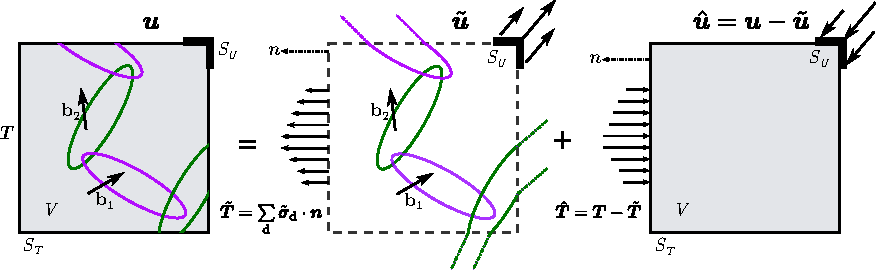
\includegraphics[width=\linewidth]{fem_ddd.pdf}
			\caption[Coupling Discrete Dislocation Dynamics to Finite Element Methods.]{The \kwd{dl} ensemble in a volume $ V $ is bounded by surface $ S $. First, the traction field $ \sum_{\textrm{d}} \tns{\tilde{\sigma}}_{\textrm{d}} $ due to the \kwd{dl} ensemble is evaluated at the surface. Then, a traditional \kwd{fem} or \kwd{bem} calculates the image traction field $ \tns{\hat{\sigma}} \times \vec{n} $. Which is then fed back to the \kwd{ddd} problem to evolve the \kwd{dl} positions and repeat the cycle. Image edited from \cite{analytical_integration_of_the_forces_induced_by_dislocations_on_a_surface_element}.}
			\label{f:fem_ddd}
		\end{figure}